\documentclass[jou, apacite]{apa6}
\usepackage{threeparttable}
\usepackage{amsmath}
\usepackage{amsfonts}
\usepackage{amssymb}
\usepackage{bm}
\usepackage{graphicx}
\graphicspath{ {./Images/} }

\raggedbottom

\begin{document}
\title{Evaluating Main Effects in the Generalized Linear Model}
\shorttitle{Interpreting GLM Main Effects}

\fiveauthors{Max A. Halvorson}{Xiaolin Cao}{Connor J. McCabe}{Dale S. Kim}{Kevin M. King}
\fiveaffiliations{University of Washington}{University of Washington}{University of Washington}{University of California, Los Angeles}{University of Washington}

\abstract{}

\keywords{count models, logistic regression, generalized linear models, data visualization}

\rightheader{Evaluating GLM Main Effects}
\leftheader{Halvorson, Cao, McCabe, Kim, and King}

\maketitle

\section{Introduction}

Despite widespread use of count and binary outcome models, very few (lit search results) researchers report model results in terms of the quantities they set out to understand. We randomly sampled X number of articles published between 200X and 200X, using the same criteria as Norton (2004) and/or Brambor, Clark, \& Golder (2006). Our results indicated that BLAH.

In count models, this entails reporting predicted counts, and in binary outcome models, this entails reporting predicted probabilities of an event occurring. We advocate for presenting quantities of interest directly, as models are readily able to output direct predictions of these quantities. Thoughtful graphical and tabular presentation of data can facilitate intuition even when models are complicated, and present a richer source of information than single parameters. 

\section{Independent Interpretation of Single Coefficients does not Characterize Models Well}
In examining predicted counts and probabilities, it becomes apparent that the single parameters reported in GzLMs do not map onto relationships between predictors and outcomes as readily as they seem to. In fact, further analysis of these parameters reveals that even their transformed versions, such as odds ratios and rate ratios, a) do not represent constant first differences, and b) do not represent effects that are conditionally independent from one another, as in OLS linear regression. To show that these two properties hold for binary outcome and count models, we present a simulated-data example with two predictors for each model below. 




\section{Binary Outcome Models}

%Stolen directly from Dale's paper for now
The mathematical formulation for any GLM can be shown as:

\begin{equation}
g(\mathbb{E}[Y|\bm{X}]) = \bm{X} \beta ,
\end{equation}

where $g(\cdot)$ is the link function, $\bm{X}\beta$ are linear predictors, and $\mathbb{E}[Y|\bm{X}]$ is taken with respect to the probability distribution.

\subsection{The Logistic Model}

The logistic model is formulated as follows:

\begin{equation} \label{log1}
\pi_i = \dfrac{\exp (X \bm{\beta})}{1 + \exp (X \bm{\beta})},
\end{equation}

First differences are not constant.


\begin{figure}[h]
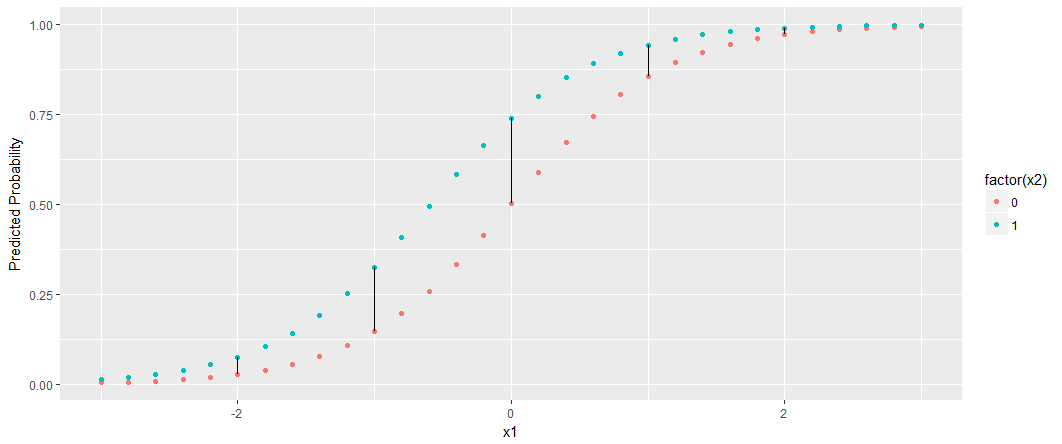
\includegraphics[width=0.5\textwidth]{LogisticFirstDiff.png}
\end{figure}

\section{Count Models}

\subsection{The Poisson Model}

\begin{equation} \label{pois1}
\mathbb{P}(Y_i = y_i|x_i) = \dfrac{\lambda_i^{y_i}e^{-y_i}}{y_i!}, \quad\text{for } y_i = 0, 1, \dots
\end{equation}
\begin{equation} \label{pois2}
\mathbb{E}[Y_i|x_i] = \lambda_i = \exp (x_i^T \bm{\beta})
\end{equation}

\begin{figure}[h]
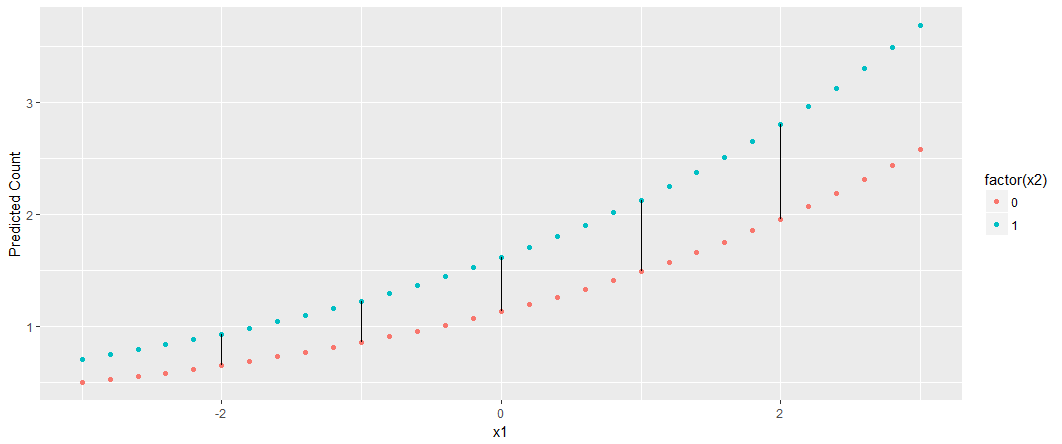
\includegraphics[width=0.5\textwidth]{PoissonFirstDiff.png}
\end{figure}

\subsection{The Negative Binomial Model}

negative binomial formulation:

\begin{equation}
\mathbb{P}(Y_i = y_i | x_i) = \dfrac{\Gamma(y_i + \theta)}{\Gamma(\theta)y_i!}
  \cdot
  \dfrac{\lambda_i^{y_i}\theta^{\theta}}{(\lambda_i + \theta)^{(y_i + \theta)}},
\end{equation}
\begin{equation}
\mathbb{E}[Y_i|x_i] = \lambda_i = \exp (x_i^T \bm{\beta}),
\end{equation}
where $\Gamma(\cdot)$ is the gamma function and $\theta$ is a constant shape parameter.

The negative binomial model is a generalization of the poisson model with an extra parameter, allowing for non-constant exposure. As such, the properties of non-constant first differences and non-independence of regression coefficients applies. 


\subsection{The Hurdle Model}

hurdle model formulation:

\begin{equation}
\mathbb{P}(Y_i = y_i|x_i) =
  \begin{cases}
    \pi_i, & \text{if } y_i = 0 \\
    (1 - \pi_i)\mathbb{P}_c(Y_i = y_i|x_i), & \text{if } y_i = 1, 2, \dots
  \end{cases}
\end{equation}
\begin{equation}
\pi_i = \dfrac{\exp (x_i^T \bm{\beta}_{\pi})}{1 + \exp (x_i^T \bm{\beta}_{\pi})},
\end{equation}
\begin{equation}
\mathbb{E}[Y_i|x_i] = (1 - \pi_i)\mathbb{E}_c[Y_i|x_i], % Placeholder - Verify
\end{equation}
where $\pi_i$ is once again assumed to be a Bernoulli parameter with logit link.

The hurdle model is a piecewise model involving 1) a logistic regression portion which accounts for zeros and 2) a poisson (or other count) model to account for non-zero values. Hurdle models assume a two-step data generating processes: one that explains whether an observation was a 0 or a positive count (portion 1), and one that predicts that positive count (2). As these models are composed of the aforementioned models, the properties of non-constant first differences and non-independence of regression coefficients applies. 

\subsection{The Zero-Inflated Model}

zero-inflated model formulation:
\begin{equation}
\mathbb{P}(Y_i = y_i|x_i) =
  \begin{cases}
    \pi_i + (1 - \pi_i)\mathbb{P}_c(Y_i = 0|x_i), & \text{if } y_i = 0 \\
    (1 - \pi_i) \mathbb{P}_c(Y_i = y_i|x_i), & \text{if } y_i = 1, 2, \dots
  \end{cases}
\end{equation}
\begin{equation}
\pi_i = \dfrac{\exp (x_i^T \bm{\beta}_{\pi})}{1 + \exp (x_i^T \bm{\beta}_{\pi})},
\end{equation}
\begin{equation}
\mathbb{E}[Y_i|x_i] = (1 - \pi_i)\mathbb{E}_c[Y_i|x_i], % Verify this.
\end{equation}
where $\pi_i$ refers to the probability of an excess zero and $\mathbb{E}_c[Y_i|x_i]$ is the expectation with respect to $\mathbb{P}_c(Y_i|x_i)$.

The zero-inflated model is a mixture model involving the poisson model (or another count model), which accounts for two processes of generating zeros. Structural zeros, represented by the first term in part 1 of the piecewise function, occur when zeros are thought to be the result of a lack of exposure. Sampling zeros, represented by the second term in part 1 of the piecewise function, are zeros that were sampled from the full count distribution. Positive counts are modeled by part 2 of the piecewise function. As such, the properties of non-constant first differences and non-independence of regression coefficients applies. 


\begin{equation} \label{zip1}
\mathbb{P}(Y_i = y_i|x_i) =
  \begin{cases}
    \pi_i + (1 - \pi_i)e^{-y_i}, & \text{if } y_i = 0 \\
    (1 - \pi_i) \dfrac{\lambda_i^{y_i}e^{-y_i}}{y_i!}, & \text{if } y_i = 1, 2, \dots
  \end{cases}
\end{equation}
\begin{equation} \label{zip2}
\pi_i = \dfrac{\exp (x_i^T \bm{\beta}_{\pi})}{1 + \exp (x_i^T \bm{\beta}_{\pi})},
\end{equation}
\begin{equation} \label{zip3}
\lambda_i = \exp (x_i^T \bm{\beta}_{\lambda}),
\end{equation}
\begin{equation} \label{zip4}
\mathbb{E}[Y_i|x_i] = (1 - \pi_i)\lambda_i,
\end{equation}
where $\pi_i$ refers to the probability of an excess zero as before.


\section{}
When presenting results, is important to recall that the choice of covariate levels chosen as 0 values can influence the interpretation of results to the majority of readers, who do not have time to probe a model fully. 

We propose that research producers should choose their covariate values thoughtfully. 

In order to characterize an effect accurately, researchers may have to probe an effect at multiple covariate levels, even when no interactions are included in the model.

\section{Recommendations for Model Reporting: Tables and Graphics}
\subsection{Binary Outcome Data}
Table of first differences with covariate values made explicit

Graphic of first differences for some X1 and X2 of interest	

Real data example???

Show graphs from InterActive? With uncertainty.

\subsection{Count Data}
Table of first differences with covariate values made explicit

Graphic of first differences for some X1 and X2 of interest

Real data example???

Show graphs from InterActive? With uncertainty.

\end{document}
